\documentclass[cmbright]{staauth}

\usepackage{amssymb, amsmath, latexsym, array, morefloats, epsfig, rotating, graphicx}
\usepackage{subfigure, url, mathtools, enumerate, wasysym, threeparttable, lscape}
\usepackage{natbib,color}
\usepackage{bm, bbm,epstopdf}
\usepackage{xr, zref, hyperref}
\usepackage{cprotect}

\newcommand{\var}{\mathrm{var}}
\newcommand{\cov}{\mathrm{cov}}
\newcommand{\E}{\mathrm{E}}
\newcommand{\tr}{\mathrm{tr}}

% if variable blind is undefined, assume it is 0
\makeatletter
\@ifundefined{blind}{\def\blind{0}}{}
\makeatother

% if not blinded, reference unblinded appendix
\if0\blind
{
  \externaldocument{psokrigingapp}
}\fi

% if blinded, reference blinded appendix
\if1\blind
{
  \externaldocument{psokrigingappblind}
}\fi


\begin{document}
\if0\blind
{
  \runninghead{M Simpson}{AT-PSO for Spatial Design}
  \title{Adaptively-Tuned Particle Swarm Optimization with Application to Spatial Design}
  \author{Matthew Simpson\affil{a}\corrauth}
%, Christopher K. Wikle\affil{a}, Scott H. Holan\affil{a}}
  \address{\affilnum{a}Department of Statistics, University of Missouri,\\
    146 Middlebush Hall, Columbia, MO 65211-6100}
  \corremail{themattsimpson@gmail.com}
  \received{00 Month Year}
  \accepted{00 Month Year}
}\fi

\if1\blind
{
  \runninghead{}{AT-PSO for Spatial Design}
  \title{Adaptively-Tuned Particle Swarm Optimization with Application to Spatial Design}
  \author{}
  \address{}
  \corremail{}
  \received{}
  \accepted{}
}\fi
\begin{abstract}
Particle swarm optimization (PSO) algorithms are a class of heuristic optimization algorithms that are especially attractive for complex optimizations problems. We propose using PSO in order to solve spatial design problems, e.g. choosing new locations to add to an existing monitoring network. To this end, we introduce a new class of PSO algorithms, called adaptively-tuned PSO, that perform well in a wide variety of circumstances. In order to illustrate these algorithms, we apply them to a common spatial design problem: choosing new locations to add to an existing monitoring network. Specifically, we consider a network in the Houston, TX area for monitoring ambient ozone levels, which have been linked to out-of-hostpital cardiac arrest rates \citep{ensor2013case}.
\end{abstract}
\keywords{optimization; particle swarm; geostatistics; kriging; optimal design, spatial prediction}
\maketitle

\section{Introduction}
PSO refers to a large class of heuristic optimization algorithms that that rely on an analogy with animal flocking behavior and are typically more robust than many alternatives \citep{clerc2002particle,blum2008swarm,clerc2010particle}. This robustness makes them attractive for more difficult optimization problems, especially when near optimal solutions are tolerable. We introduce a new class of PSO algorithms, called adaptively tuned PSO (AT-PSO), which exploit an analogy with a class of adaptive Markov chain Monte Carlo algorithms in order to tune a crucial parameter of the PSO algorithm adaptively based on the state of the particle swarm. We show that the resulting algorithms tend to be superior to many PSO alternatives. Additionally, we illustrate several PSO algorithms by applying them to choosing a set of new monitoring locations for ozone in Harris County, Texas, where Houston is located. Ambient ozone levels have been linked to cardiac arrest \citep{ensor2013case}, and ozone monitoring is an essential tool for determining when and where populations are at risk.

Section \ref{sec:pso} introduces various PSO and AT-PSO algorithms, and briefly discusses the results of an extended simulation study comparing them. Section \ref{sec:spatialdesign} introduces the generic spatial design problem and the Houson area ozone problem as an instance of that problem, and compares several PSO algorithms and some alternatives to solving the problem. Finally, Section \ref{sec:discuss} discusses our results and concludes.

\section{Particle swarm optimization}\label{sec:pso}
We briefly describe PSO here; refer to \citet{blum2008swarm} for a comprehensive introduction, \citet{clerc2010particle} for details, and \citet{clerc2011spso} for good default versions of the algorithm. Suppose that we wish to minimize some objective function $Q(\bm{\theta}):\Re^D\to\Re$. Let $i=1,2,\dots,n$ index a set of particles over time, $k=1,2,\dots,K$, where in every period each particle consists of a location $\bm{\theta}_i(k)\in \Re^D$, a velocity $\bm{v}_i(k) \in \Re^D$, a personal best location $\bm{p}_i(k)\in\Re^D$, and a group best location $\bm{g}_i(k)\in\Re^D$. Here we mean ``best'' in the sense of minimizing $Q$, so $Q(\bm{p}_i(k)) \leq Q(\bm{\theta}_i(l))$ for any $k\geq l$. The group best location is defined with respect to some neighborhood $\mathcal{N}_i$ of particle $i$; that is, $\bm{g}_i(k) = \arg\min_{\{\bm{p}_j(k)|j\in\mathcal{N}_i\}}Q(\bm{p}_j(k))$. In the simplest case where the entire swarm is the neighborhood of each particle, $\bm{g}_i(k)\equiv \bm{g}(k) = \arg\min_{\{\bm{p}_j(k)|j\in 1:n\}}Q(\bm{p}_j(k))$. The generic PSO algorithm updates each particle $i$ as follows:
\begin{align}\label{eq:pso}
\bm{v}_i(k+1) &= \omega \bm{v}_i(k) + \phi_1 \bm{r}_{1i}(k)\circ\{\bm{p}_i(k) - \bm{\theta}_i(k)\} + \phi_2 \bm{r}_{2i}(t)\circ\{\bm{g}_i(k) - \bm{\theta}_i(k)\},\nonumber\\
\bm{\theta}_i(k+1) &= \bm{\theta}_i(k) + \bm{v}_i(k+1),\nonumber\\
\bm{p}_i(k+1) &= \begin{cases} \bm{p}_i(k)   & \mbox{if }\  Q(\bm{p}_i(k)) \le Q(\bm{\theta}_i(t + 1))\\
                               \bm{\theta}_i(k+1) & \mbox{otherwise},
\end{cases}\nonumber\\
\bm{g}_i(k+1) &= \arg\min_{\{\bm{p}_j(k+1)|j\in\mathcal{N}_i\}}Q(\bm{p}_j(k+1)),
\end{align}
where $\circ$ denotes the Hadamard product (element-wise product), $\bm{r}_{1i}(k)$ and $\bm{r}_{2i}(k)$ are each vectors of $D$ random variates independently generated from the $U(0,1)$ distribution, and $\omega>0$, $\phi_1>0$, and $\phi_2>0$ are user-defined parameters. The term $\omega \bm{v}_i(k)$ controls the particle's tendency to keep moving in the direction it is already going, so $\omega$ is called the inertia parameter. Similarly $\phi_1 \bm{r}_{1i}(k)\circ\{\bm{p}_i(k) - \bm{\theta}_i(k)\}$ controls the particle's tendency to move towards its personal best location while $\phi_2 \bm{r}_{2i}(k)\circ\{\bm{g}_i(k) - \bm{\theta}_i(k)\}$ controls its tendency to move toward its group best location, so $\phi_1$ and $\phi_2$ are called the cognitive correction factor and social correction factor, respectively \citep{blum2008swarm}. This version of PSO is equivalent to \citet{clerc2002particle}'s constriction type I particle swarm, though there are many other variants. One default choice sets $\omega = 0.7298$ and $\phi_1 = \phi_2 = 1.496$ \citep{clerc2002particle} while another sets $\omega = 1/(2\ln 2)\approx 0.721$ and $\phi_1=\phi_2=1/2 + \ln 2\approx 1.193$ \citep{clerc2006stagnation}.

Any PSO variant can also be combined with various neighborhood topologies that control how the particles communicate to each other. The default global topology allows each particle to see each other particle's previous best location for the social components of their respective velocity updates, but this can cause inadequate exploration and premature convergence. Alternative neighborhood topologies limit how many other particles each particle can communicate with. We use a variant of the stochastic star topology \citep{miranda2008stochastic}. Each particle informs itself and $k$ random particles from the swarm, sampled with replacement during initialization of the algorithm. On average this implies that each particle is informed by $k$ particles, though a small number of particles will often be informed by many of the other particles

Bare bones PSO (BBPSO) is a variant of PSO introduced by \citet{kennedy2003bare} that strips away the velocity term. Let $\theta_{ij}(k)$ denote the $j$th coordinate of the position for the $i$th particle in period $t$, and similarly for $p_{ij}(k)$ and $g_{ij}(k)$. Then the BBPSO algorithm obtains a new position coordinate $\theta_{ij}$ via
\begin{align}\label{eq:bbpso}
\theta_{ij}(k+1) \sim N\left(\frac{p_{ij}(k) + g_{ij}(k)}{2}, |p_{ij}(k) - g_{ij}(k)|^2\right).
\end{align}
The updates of $\bm{p}_i(k)$ and $\bm{g}_i(k)$ are the same as in \eqref{eq:pso}. We explain the essential ideas of PSO and BBPSO in this section, though several modifications can be made to improve performance. Appendix \ref{app:psodetail} details each of the modifactions we use, most of which come from \citet{clerc2011spso}. In the next two subsections we introduce adaptively-tuned BBPSO and adaptively-tuned PSO respectively. Both of these algorithms can be combined with the various modifications we discuss in Appendix \ref{app:psodetail}.

\subsection{Adaptively tuned BBPSO}\label{subsec:ATBBPSO}
BBPSO adapts the size effective search space of the swarm over time through the variance term, $|p_{ij}(k) - g_{ij}(k)|^2$. As the personal best locations of the swarm move closer together, these variances decrease and the swarm explores locations which are closer to known high value areas in the space. This behavior is desirable, but the adaptation is forced to occur only through personal and group best locations. In order to allow the algorithm to adapt in a more flexible manner, we modify the BBPSO variance to $\sigma^2(k)|p_{ij}(k) - g_{ij}(k)|^2$ and tune $\sigma^2(k)$ in a manner similar to adaptive random walk Metropolis MCMC algorithms \citep{andrieu2008tutorial}. Define the improvement rate of the swarm in period $t$ as $R(k) = \#\{i:Q(\bm{p}_i(k))> Q(\bm{p}_i(k-1))\}/n$ where $\#A$ is the number of members of the set $A$, and let $R^*$ denote the target improvement rate. Then adaptively tuned BBPSO (AT-BBPSO) updates the swarm's personal best and group best locations as in \eqref{eq:pso}, then updates particle locations as follows:
\begin{align}\label{eq:at-bbpso}
\theta_{ij}(k+1) &\sim t_{df}\left(\frac{p_{ij}(k) + g_{ij}(k)}{2}, \sigma^2(k)|p_{ij}(k) - g_{ij}(k)|^2\right),\nonumber\\
\log \sigma^2(k+1) &= \log\sigma^2(k) + c\times\{R(k+1) - R^*\},
\end{align}
where $df$ is a user chosen degrees of freedom parameter and $c$ is another user chosen parameter that controls the speed of adaptation. We use a $t$ kernel instead of a Gaussian in order to allow for more flexibility, and we find $df=1$ appears to combine well with adaptively tuning $\sigma^2(k)$. Setting the target rate from $R^*=0.3$ to $R^*=0.5$ tends to yield AT-BBPSO algorithms which work well, which is unsurprising given the connection to adaptive random walk Metropolis \citep{gelman1996efficient}. The parameter $c$ controls the speed of adaptation so that larger values of $c$ mean the algorithm adapts $\sigma^2(k)$ faster. We find that $c=0.1$ works well, though anything within an order of maginitude yields similar results. We use $\sigma^2(0)=1$ to initialize the algorithm at the standard BBPSO algorithm. Optimal selection of the tuning parameters, in particular $c$, is a subject of future research.

Both using a $t$ kernel and adding a fixed scale parameter have been discussed in the BBPSO literature, but as \citet{kennedy2003bare} notes, something about setting $\sigma^2=1$ is special that causes the algorithm to work well. A similar BBPSO algorithm from \citet{hsieh2010modified} sets $\sigma^2<1$ for an initial set of iterations, then eventually sets $\sigma^2=1$. The authors alo suggest dynamically adjusting $\sigma^2$ in the early stage of the algorithm before they are set to one, but give no suggestion for how to do this. AT-BBPSO is able to adapt its value on the fly based on local knowledge about the objective function. If too much of the swarm is failing to find new personal best locations, AT-BBPSO proposes new locations closer to known high value areas. If too much of the swarm is improving, AT-BBPSO proposes bolder locations in an effort to make larger improvements. This ability to adapt to local information about the objective function allows AT-BBPSO to more quickly traverse the search space towards the global optimum, though by using local information AT-BBPSO does risk premature convergence to a local optimum. The adaptively tuned component of AT-BBPSO can also be combined with most BBPSO variants, some of which are outlined in Appendix \ref{app:psodetail}. In Appendix \ref{app:psocompare} we conduct a simulation study on several test functions that compares AT-BBPSO variants to other PSO and BBPSO variants in order to justify the parameter settings discussed above and demonstrate AT-BBPSO variants are attractive PSO algorithms.

\subsection{Adaptively-tuned PSO}\label{sec:AT-PSO}
In AT-BBPSO variants, the parameter $\sigma(k)$ partially controls the effective size of the swarm's search area, and we increase or decrease $\sigma(k)$ and consequently the search area depending on how much of the swarm is finding new personal best locations. In standard PSO the inertia parameter, denoted by $\omega$ in \eqref{eq:pso}, is roughly analogous to $\sigma^2$ in BBPSO. It controls the effective size of the swarm's search area by controlling how the magnitude of the velocities evolve over time. In AT-BBPSO we use an analogy with tuning a random walk Metropolis-Hastings MCMC algorithm in order to build intuition about how to tune $\sigma(k)$. The analogy is much weaker in this case; nonetheless, the same mechanism works well to tune $\omega(k)$. Formally, AT-PSO updates personal and group best locations as in \eqref{eq:pso} and updates $\omega(k)$ and particle locations as follows:
\begin{align}\label{eq:atpso}
\bm{v}_i(k+1) &= \omega(k+1) \bm{v}_i(k) + \phi_1 \bm{r}_{1i}(k)\circ\{\bm{p}_i(k) - \bm{\theta}_i(k)\} + \phi_2 \bm{r}_{2i}(k)\circ\{\bm{g}_i(k) - \bm{\theta}_i(k)\},\nonumber\\
\bm{\theta}_i(k+1) &= \bm{\theta}_i(k) + \bm{v}_i(k+1),\nonumber\\
\log\omega(k+1)& = \log\omega(k) + c\times\{R(k+1) - R^*\},
\end{align}
where $R(k)$ is the improvement rate of the swarm in iteration $t$, $R^*$ is the target improvement rate, and $c$ controls how much $R(k)$ changes on a per iteration basis. Again, we find that target rates from $R^*=0.3$ to $0.5$ work well for AT-PSO. The value of $c$ controls the speed of adaptation. We use $c=0.1$ as a default value and in simulations (not reported here), we find that the gains from optimizing $c$ appear to be small. However, optimal selection of these tuning parameters is a subject of future research. The adaptive tuning piece of this algorithm can be combined with almost any PSO variant, and Appendix \ref{app:psodetail} describes the various modifications to the standard PSO algorithm we employ, both in conjuction with AT and without it.

The idea of time-varying $\omega(k)$ has been in the PSO literature for some time. An early suggestion was to set $\omega(0)=0.9$ and deterministically decrease it until it reaches $\omega(k)=0.4$ after the maximum number of iterations allowed \citep{eberhart2000comparing}. In particular, \citet{tuppadung2011comparing} suggest defining $\omega(k)$ via the parameterized inertia weight function $\omega(k) = 1/\left[1 + (t/\alpha)^{\beta}\right]$ where $\alpha$ and $\beta$ are user-defined parameters. Roughly, $\alpha$ controls how low $\omega(k)$ can go and $\beta$ controls how fast it gets there, so $\alpha$ and $\beta$ can be thought of as intercept and slope parameters respectively. The suggestion in \citet{tuppadung2011comparing} is to set $\alpha$ to a small fraction of the total amount of iterations in which the algorithm is allowed to run (e.g., 10\% or 20\%), and set $\beta$ between one and four. We call this type of PSO algorithm deterministic inertia PSO (DI-PSO).

DI-PSO tends to improve on standard PSO if $\omega(k)$'s progression is set appropriately, but this can be difficult and often depends on the problem. A priori it may not be clear exactly which approach is best for any given problem, so an automatic method is desirable. A major strength of AT-PSO relative to DI-PSO and standard PSO is that AT-PSO can increase $\omega(k)$ when information from the swarm suggests there is an unexplored high value region of the space. Just like in AT-BBPSO, this mechanism provides a way for the swarm to adapt its behavior on the fly based on local conditions and speed up convergence by allowing the particles that do improve to make larger improvements, but it can also cause premature convergence to a local optimum. While DI-PSO monotonically decreases $\omega(k)$ toward some minimum value, AT-PSO typically oscillates $\omega(k)$ so that the algorithm alternates between periods of exploration and exploitation.

Another similar algorithm comes from \citet{zhang2003adaptive}. In their algorithm, $\omega$ is constant while $\phi_1$ and $\phi_2$ not only vary across time, but also across the swarm. Then each particle adapts its values of $\phi_1$ and $\phi_2$ based on how much it improves on its personal best location. The key difference is that the adaptation is local to each specific particle while in AT-PSO the adaptation is global. AT-PSO takes into account less information by ignoring local conditions of the particles, but the adaptation scheme is simpler and the analogy with adaptive random walk Metropolis helps build intuition for choosing sensible default parameter values.

The simulation study in Appendix \ref{app:psocompare} includes several AT-PSO algorithms and demonstrates some of the behavior detailed above. Further, it shows that AT-PSO is often an attractive optimization algorithm relative to other PSO options.

\section{The Spatial Design Problem}\label{sec:spatialdesign}
Suppose we are interested predicting some spatially indexed response variable $Y(\bm{u})$, $\bm{u}\in \mathcal{D}\subseteq \Re^2$ at a set of target locations $\bm{t}_1, \bm{t}_2, \dots, \bm{t}_{N_t}\in\mathcal{D}$. Let $\bm{s}_1, \bm{s}_2, \dots, \bm{s}_{N_s}\in\mathcal{D}$ denote a set of $N_s$ fixed sampling locations within the spatial domain. The design problem is to add $N_d$ new sampling locations in order to optimize the amount we learn about $Y(\bm{u})$ at the target locations. Let $\bm{d}_1, \bm{d}_2, \dots, \bm{d}_{N_d}\in\mathcal{D}$ denote a set of candidate design points and suppose that $Y(\bm{u})$ is a geostatistical process with mean function $\mu(\bm{u})=\bm{x}(\bm{u})'\bm{\beta}$ for some covariate $\bm{x}(\bm{u})$ known at every point in $\mathcal{D}$ and some covariance function $C(\bm{u}, \bm{v})$ for $\bm{u},\bm{v}\in\mathcal{D}$. Not all covariates can be known a priori at every point in the spatial domain; however, covariates that are known functions of the location satisfy this constraint. Once the design points are selected, we observe $Z(\bm{d}_i)$ for $i=1,2,\dots,N_d$ and $Z(\bm{s}_i)$ for $i=1,2,\dots,N_s$ where $Z(\bm{u}) = Y(\bm{u}) + \varepsilon(\bm{u})$ and $\varepsilon(\bm{u})$ is mean zero white noise with variance $\tau^2$, representing measurement error. Typically $\bm{\beta}$, $\tau^2$, and $C(.,.)$ are unknown and must be estimated, though for now we will treat them as known.

To completely specify the problem we need to define an informative design criterion. Intuitively, the larger the mean square prediction error (MSPE), i.e. the kriging variance, is at each of the target locations, the less information we have about $Y(\bm{u})$ at those locations. A common design criterion is to optimize is some function of these variances, e.g. to minimize the mean kriging variance or the maximum kriging variance over all target locations. These criteria are somewhat naive since they they ignore parameter uncertainty, and taking that into account will often change the optimal design \citep{zimmerman2006optimal}.

\subsection{Universal Kriging}
In universal kriging, $C(.,.)$ and $\tau^2$ are treated as known while $\bm{\beta}$ is treated as a parameter that needs to be estimated. Let $\bm{Z}$ be the vector of $Z(\bm{s}_i)$s and $Z(\bm{d}_i)$s, $\bm{X}$ denote the corresponding stacked $\bm{x}(\bm{s}_i)'$s and $\bm{x}(\bm{d}_i)'$s, $\bm{C}_Z = \cov(\bm{Z})$ where $\cov[Z(\bm{u}), Z(\bm{v})] = C(\bm{u},\bm{v}) + \sigma^2_\varepsilon 1(\bm{u} = \bm{v})$, and $\bm{c}_Y(\bm{t}_i) = \cov[Y(\bm{t}_i), \bm{Z}]$ where $\cov[Y(\bm{t}_i), Z(\bm{u})] = C(\bm{t}_i, \bm{u})$. The universal kriging predictor of $Y(\bm{t}_i)$ is $\widehat{Y}_{uk}(\bm{t}_i;\bm{d}) = \bm{x}(\bm{t}_i)'\widehat{\bm{\beta}}_{gls} + \bm{c}_Y(\bm{t}_i)'\bm{C}_Z^{-1}(\bm{Z} - \bm{X}\widehat{\bm{\beta}}_{gls})$ and the MSPE of $\widehat{Y}_{uk}(\bm{t}_i)$ is
\begin{align*}
\sigma_{uk}^2(\bm{t}_i;\bm{d}) &= C(\bm{t}_i, \bm{t}_i) - \bm{c}_Y(\bm{t}_i)'\bm{C}_Z^{-1}\bm{c}_Y(\bm{t}_i)  \\
& + [\bm{x}(\bm{t}_i)  - \bm{X}'\bm{C}_Z^{-1}\bm{c}_Y(\bm{t}_i)]'[\bm{X}'\bm{C}_Z^{-1}\bm{X}]^{-1}[\bm{x}(\bm{t}_i)  - \bm{X}'\bm{C}_Z^{-1}\bm{c}_Y(\bm{t}_i)].
\end{align*}
where $\widehat{\bm{\beta}}_{gls} = [\bm{X}'\bm{C}_Z^{-1}\bm{X}]^{-1}\bm{X}'\bm{C}_Z^{-1}\bm{Z}$ is the generalized least squares estimate of $\bm{\beta}$ \citep[Section~4.1.2]{cressie2011statistics}. To avoid clutter we drop the explicit dependence on $\bm{d}$ in these equations, but $\bm{c}_Y(\bm{t}_i)$, $\bm{C}_Z$, $\bm{Z}$, $\bm{X}$, and $\widehat{\bm{\beta}}_{gls}$ all depend on $\bm{d}$. The mean universal kriging variance is given by $\overline{Q}_{uk}(\bm{d}) = \frac{1}{N_t}\sum_{i}^{N_t}\sigma^2_{uk}(\bm{t}_i;\bm{d})$ while the maximum universal kriging variance is given by $Q_{uk}^*(\bm{d}) = \max_{i=1,2\dots,N_t}\sigma^2_{uk}(\bm{t}_i;\bm{d})$. \cite{zimmerman2006optimal} finds that the optimal design under both criteria is highly dependent on the class of mean function of the geostatistical process. In practice we are often interested in predicting at the entire spatial domain rather than a finite set of target locations. This changes the mean and maximum kriging variances to $\overline{Q}_{uk}(\bm{d}) = \frac{1}{|\mathcal{D}|}\int_{\mathcal{D}}\sigma^2_{uk}(\bm{u};\bm{d})d\bm{u}$ and $Q_{uk}^*(\bm{d}) = \max_{\bm{u}\in\mathcal{D}}\sigma^2_{uk}(\bm{u};\bm{d})$ respectively. We can approximate both of these with a large but finite sample of target locations from $\mathcal{D}$ or a large fixed grid in $\mathcal{D}$.

\subsection{Parameter Uncertainty Kriging}
Assuming that all covariance function parameters are known, the MSPE from kriging at an arbitrary location $\bm{u}$ is $\sigma_{uk}^2(\bm{u})$. This underestimates the MSPE when those parameters must be estimated. An approximation of the correct MSPE, which we call the parameter uncertainty kriging variance (PUK variance), is given by \citep{zimmerman1992mean,abt1999estimating}
\begin{align*}
\E[Y(\bm{u}) - \widehat{Y}_{uk}(\bm{u})]^2 \approx \sigma^2_{puk}(\bm{u};\bm{d},\widehat{\bm{\theta}}) = \sigma^2_{uk}(\bm{u};\bm{d},\widehat{\bm{\theta}}) + \tr[\bm{A}(\bm{u};\bm{d},\widehat{\bm{\theta}})\bm{I}^{-1}(\bm{d},\widehat{\bm{\theta}})]
\end{align*}
where $\widehat{\bm{\theta}}$ is the maximum likelihood estimate of $\bm{\theta}$ from previously observed data, $\bm{I}^{-1}$ is the inverse Fisher information (FI) matrix, and $\bm{A} = \var[\partial \widehat{Y}_{uk} /\partial \bm{\theta}]$. The $ij$th element of the FI matrix can be derived as $\tr\left(\bm{C}_Z^{-1}\frac{\partial\bm{C}_Z}{\partial\theta_i}\bm{C}_Z^{-1}\frac{\partial\bm{C}_Z}{\partial\theta_j}\right)$ while $\bm{A}$ can be derived using elementary matrix calculus. From these we define the mean and maximum  PUK variances as $\overline{Q}_{puk}(\bm{d}) = \frac{1}{N_t}\sum_{i}^{N_t}\sigma^2_{puk}(\bm{t}_i;\bm{d})$ and $Q_{puk}^*(\bm{d}) = \max_{i=1,2\dots,N_t}\sigma^2_{puk}(\bm{t}_i;\bm{d})$ respectively.

% To derive $\bm{A}$ note that $\widehat{Y}_{uk}$ can be rewritten as
% \begin{align*}
% \widehat{Y}_{uk}(\bm{u}) = \bm{x}(\bm{u})'\bm{U}'\bm{Z} + \bm{c}_Y(\bm{u})'\bm{V}'\bm{Z}
% \end{align*}
% where $\bm{U} = \bm{C}_Z^{-1}\bm{X}(\bm{X}'\bm{C}_Z^{-1}\bm{X})^{-1}$ and $\bm{V} = \bm{C}_Z^{-1} - \bm{U}\bm{X}'\bm{C}_Z^{-1}$. Then elementary matrix calculus yields
% \begin{align*}
% \frac{\partial \widehat{Y}_{uk}(\bm{u})}{\partial \theta_i} &= \bm{x}(\bm{u})'\frac{\partial \bm{U}}{\partial \theta_i}'\bm{Z} + \frac{\partial \bm{c}_Y(\bm{u})}{\partial \theta_i}'\bm{V}'\bm{Z} + \bm{c}_Y(\bm{u})'\frac{\partial \bm{V}}{\partial \theta_i}'\bm{Z}\\
% &= \left[-\bm{V}\frac{\partial \bm{C}_Z}{\partial \theta_i}\bm{U}\bm{x}(\bm{u}) - \bm{V}\frac{\partial \bm{C}_Z}{\partial \theta_i}\bm{V}\bm{c}_Y(\bm{u}) + \bm{V}\frac{\partial \bm{c}_Y(\bm{u})}{\partial \theta_i}\right]'\bm{Z}\\
% &\equiv\bm{\delta}_i'\bm{Z}.
% \end{align*}
% Then
% \begin{align*}
% \bm{A} = \var\left[\frac{\partial \widehat{Y}_{uk}(\bm{u})}{\partial \bm{\theta}}\right] = \var[\bm{\Delta}'\bm{Z}] = \bm{\Delta}'\bm{C}_Z^{-1}\bm{\Delta}
% \end{align*}
% where $\bm{\Delta} = (\bm{\delta}_1, \bm{\delta}_2, \dots, \bm{\delta}_p)$.
\subsection{Houston Ozone Monitoring}\label{sec:houston}
The Texas Commission on Environmental Quality (TCEQ) publishes a variety of environmental data for Texas, including many environmental indicators that directly relate to public health. We focus on ozone in the Houston-Galveston-Brazoria area. The TCEQ measures ozone at a network of monitoring locations in this area and publishes daily maximum eight-hour ozone concentrations (DM8s) in parts per billion (ppb) for each monitoring location. DM8s are computed as follows. First, the TCEQ creates publishes an hourly average (in ppb) for each monitoring location. Then an eight hour average is constructed at that location for each contiguous eight-hour period where all eight measurements were present for a given day. The maximum of these eight-hour averages for a given day is the published DM8. Days with less than 18 valid eight-hour averages have no published DM8. A 20 ppb increase in DM8 has been associated with an increased risk of out-of-hospital cardiact arrest, with a relative risk estimate of 1.039 \citep[95\% CI (1.005, 1.073);][]{ensor2013case}.

In August 2016 there were 44 active monitoring locations in the Houston-Galveston-Brazoria area. For each location $\bm{u}$ we compute the monthly average DM8, which we denote by $Z(\bm{u})$. At one location, MRM-3 Haden Road, there are two DM8 observations of 0 ppb in the month of August. We assume that these were data errors and omit them for the purposes of computing $Z(\bm{u})$ at that location. Of the 44 locations, one has 15 valid DM8 measurements of 31 possible valid measurements, another has 24 valid measurements, and the rest of the locations have at least 27 valid measurements.

The hypothetical design problem we consider is the addition of 100 new ozone monitoring locations to the Houston-Galveston-Brazoria monitoring network in Harris County, where Houston is located, with the goal of predicting ozone concentrations within Harris County. Of the 44 existing locations, 33 are already in Harris County, though the locations outside of the county are still useful for spatial prediction within Harris County.

Let $Z(\bm{u})$ denote the measured average DM8 at location $\bm{u}$ and let $Y(\bm{u})$ denote the true DM8. We assume that $Z(\bm{u})$ is a noisy Gaussian measurement of $Y(\bm{u})$; i.e., the data model is $Z(\bm{u}) \sim N[Y(\bm{u}), \tau^2]$. The parameter $\tau^2$ represents variability added due to both measurement error from the instruments and potentially sampling error from measuring DM8 on less than the full 31 days in August. At the process level, we assume that $Y(\bm{u})$ is a geostatistical process with mean function $\mu(\bm{u}) = \bm{x}(\bm{u})'\bm{\beta}$ and exponential covariance function $C(\bm{u},\bm{v}) = \sigma^2\exp(-||\bm{u} - \bm{v}||/\psi)$. We assume that any fine scale variability is measurement error and captured in the data model. We considered several possible mean functions: constant in $\bm{u}$, linear in $\bm{u}$, and quadratic in $\bm{u}$. We fit each model using maximum likelihood and found that quadratic terms were unnecessary, but linear terms did significantly help explain variation in $Y(\bm{u})$.

We use both PUK design criteria in order to choose the five new locations in Harris County: $\overline{Q}_{puk}(\bm{d})$ and $Q^*_{puk}(\bm{d})$, both defined in Section \ref{sec:spatialdesign}. We assume that the goal is the predict average DM8 in all of Harris County, so we approximate the continuous versions of $\overline{Q}_{puk}(\bm{d})$ and $Q^*_{puk}(\bm{d})$ with the finite sample versions using a grid of 1229 points, obtained by gridding up the smallest rectangle containing Harris County and throwing away all points outside of the county. We try a variety of PSO algorithms in order to select the new locations. Since the design space only allows new monitoring locations within Harris County, we modify each of the PSO algorithms we use so that any particle outside of the design space is forced to moved to the nearest point on the edge of the design space as described in Appendix \ref{app:psodetail}. Existing sampling locations outside of Harris County are still used in the estimation of the model and in the construction of the PUK variances.

Table \ref{tab:psokriging} contains the results of applying optimization algorithm to choosing the 100 new monitoring locations. In the table, PSO refers to the standard PSO algorithm with the usual velocity update and all of the other modifications listed in Appendix \ref{subapp:pso}. The CF modifier indicates that the velocity update is coordinate-free -- see Appendix \ref{subapp:pso} for details. The AT modifier indicates that $\omega(k)$ is adaptively tuned as described in Section \ref{sec:AT-PSO}. AT1 uses $R^*=0.3$ and AT2 uses $R^*=0.5$, while both use $c=0.1$ and $\omega(0) = 1.2$. We use two sets of parameter values for all of the PSO algorithms: $\phi_1^{(1)}=\phi_2^{(1)}=1.496$ (PSO1) and $\phi_1^{(2)}=\phi_2^{(2)}=\ln(2) + 1/2$ (PSO2), and when applicable the corresponding inertias are $\omega^{(1)}=0.7298$ and $\omega^{(2)}=1/(2\ln 2)$. We do not list any DI algorithms since the performed extremely poorly on this problem. All of the BBPSO algorithms we consider are AT, with AT1-BBPSO and AT2-BBPSO using the same parameter values of $R^*$, and $c$ as AT1-PSO and AT2-PSO. All BBPSO algorithms also use $df=1$, and each of the modications detailed in Appendix \ref{subapp:bbpso}. Further, the CF modifier indicates that the BBPSO algorithm uses the coordinate-free variance update and the xp modifier indicates it has a 0.5 probability of moving any given coordinate of a particle to its personal best location on that coordinate, both described in Appendix \ref{subapp:bbpso}. All of the PSO and BBPSO algorithms use either the global neighborhood topology, or the variant of the stochastic star neighborhood topology discussed in Section \ref{sec:pso} with three informants. Further, each PSO algorithm has a swarm size of 40 and is run for $K=2000$ iterations. Additionally, we employ two other classes of alternative algorithms to compare to PSO. First, we use the genetic algorithm described in \citet{hamada2001finding}, with either one or two batches ($B$), and with two possible mutation rates ($\lambda$) and two possible mutation variances ($\mu$). The genetic algorithms also use a population of 40, though they are only allowed to run for 1000 iterations so that after the initialization, the genetic algorithms use the same number of objective function evaluations as each of the PSO algorithms. Finally, we use an exchange algorithm \citep{miller1994algorithm,nychka1998design}. The exchange algorithm is commonly used in spatial and spatio-temporal design problems \citep{nychka1998design,wikle1999space,wikle2005dynamic}, and uses a discrete grid as the search space and operates by considering the neighbors of the current point. We use the target grid, $\bm{t}$, as the search space and consider tenth-order neighbors. Each algorithm was implemented in the \verb0R0 programming language \citep{R2016}.

[WAITING ON GENETIC AND EXCHANGE ALGORITHMS TO FINISH TO ADD TO THE TABLE]

% latex table generated in R 3.3.2 by xtable 1.8-2 package
% Mon Dec 12 12:38:19 2016
\begin{table}[ht]
\centering
\begingroup\scriptsize
\begin{tabular}{l|r|r}
  \multicolumn{1}{l}{\begin{tabular}{lr} $\overline{Q}_{puk}$; & Nbhd: \end{tabular}} & \multicolumn{1}{c}{Global} & \multicolumn{1}{c}{SS3} \\
  \hline
Algorithm & logpost & logpost \\
  \hline
PSO1 & 14.40 & 15.62 \\
  PSO2 & 14.45 & 14.87 \\
  PSO1-CF & 15.53 & 15.94 \\
  PSO2-CF & 15.77 & 15.56 \\
   \hline
AT3-PSO1 & 14.38 & 15.25 \\
  AT3-PSO2 & 14.56 & 15.88 \\
  AT3-PSO1-CF & 15.96 & 15.98 \\
  AT3-PSO2-CF & 15.60 & 15.86 \\
   \hline
AT5-PSO1 & 14.42 & 15.70 \\
  AT5-PSO2 & 14.32 & 15.70 \\
  AT5-PSO1-CF & 15.85 & 15.96 \\
  AT5-PSO2-CF & 15.95 & 15.87 \\
   \hline
AT3-BBPSO & 14.53 & 15.72 \\
  AT3-BBPSOxp & 15.87 & 15.96 \\
  AT3-BBPSO-CF & 14.65 & 14.82 \\
  AT3-BBPSOxp-CF & 14.84 & 15.74 \\
   \hline
AT5-BBPSO & 14.65 & 15.74 \\
  AT5-BBPSOxp & 15.21 & 15.32 \\
  AT5-BBPSO-CF & 14.63 & 15.32 \\
  AT5-BBPSOxp-CF & 14.52 & 15.71 \\
   \hline
\end{tabular}
\hspace{.5cm}
\begin{tabular}{l|r|r}
\multicolumn{1}{l}{\begin{tabular}{lr} $Q^*_{puk}$; & Nbhd: \end{tabular}} & \multicolumn{1}{c}{Global} & \multicolumn{1}{c}{SS3} \\
  \hline
Algorithm & logpost & logpost \\
  \hline
PSO1 & 20.63 & 22.32 \\
  PSO2 & 21.03 & 22.63 \\
  PSO1-CF & 23.54 & 23.69 \\
  PSO2-CF & 23.16 & 23.96 \\
   \hline
AT3-PSO1 & 20.57 & 22.54 \\
  AT3-PSO2 & 23.18 & 23.14 \\
  AT3-PSO1-CF & 23.33 & 23.68 \\
  AT3-PSO2-CF & 24.02 & 23.53 \\
   \hline
AT5-PSO1 & 21.13 & 22.63 \\
  AT5-PSO2 & 22.11 & 23.28 \\
  AT5-PSO1-CF & 24.00 & 23.97 \\
  AT5-PSO2-CF & 23.63 & 23.58 \\
   \hline
AT3-BBPSO & 22.28 & 23.31 \\
  AT3-BBPSOxp & 22.19 & 23.39 \\
  AT3-BBPSO-CF & 21.33 & 23.20 \\
  AT3-BBPSOxp-CF & 22.34 & 23.44 \\
   \hline
AT5-BBPSO & 23.49 & 23.51 \\
  AT5-BBPSOxp & 23.25 & 23.15 \\
  AT5-BBPSO-CF & 21.92 & 23.33 \\
  AT5-BBPSOxp-CF & 22.76 & 23.25 \\
   \hline
\end{tabular}
\endgroup
\caption{Simulation results for $\overline{Q}_{puk}$ and $Q^*_{puk}$. See text for description.}
\label{tab:psokriging}
\end{table}

From Table \ref{tab:psokriging} we immediately see that the best performing PSO algorithms tend to use the global neighborhood topology and tend not to use the coordinate free velocity/variance update. Further the first set of parameter values tends to work the best in the PSO algorithms while in the BBPSO algorithms the non-xp variants tend to outperform the xp variants, though neither of these is universally true. For both objective functions the PSO1 algorithm with the global neighborhood topology performs the best of the non AT variants and is outperformed by few of the AT variants. The best performing algorithms for $\overline{Q}_{puk}$ are, in order, AT5-PSO2, AT3-PSO1, PSO1, AT5-PSO1, and PSO2, all with the global neighborhood topology. Similarly, the best performing algorithms for $Q^*_{puk}$ are, in order, AT3-PSO1, PSO1, PSO2, and AT5-PSO, again all with the global neighborhood topology. In Appendix \ref{app:psocompare} we found that the AT-BBPSO and AT-BBPSO-CF variants were competitive with the other PSO algorithms and in the case of the hardest problems seemed to be the best. The key seems to be that the AT-BBPSO variants are more robust to complicated objective surfaces with many local minima. When the objective surface is simpler, PSO and AT-PSO variants are more attractive and appear to converge faster. Our spatial design problem is apparently not complex enough for the advantages of AT-BBPSO to kick in. A similar dynamic seems to exist between the standard PSO and AT-PSO variants, namely that for problems that are simple enough PSO outperforms AT-PSO, but for hard enough problems AT-PSO becomes advantageous. For example in simulations not reported here, PSO1 outperforms all other algorithms when adding significantly less monitoring locations to the network, e.g. 20 or 50.

\begin{figure}
\centering
%\includegraphics[scale=.3]{../code/kriging/sig2pukboth.png}
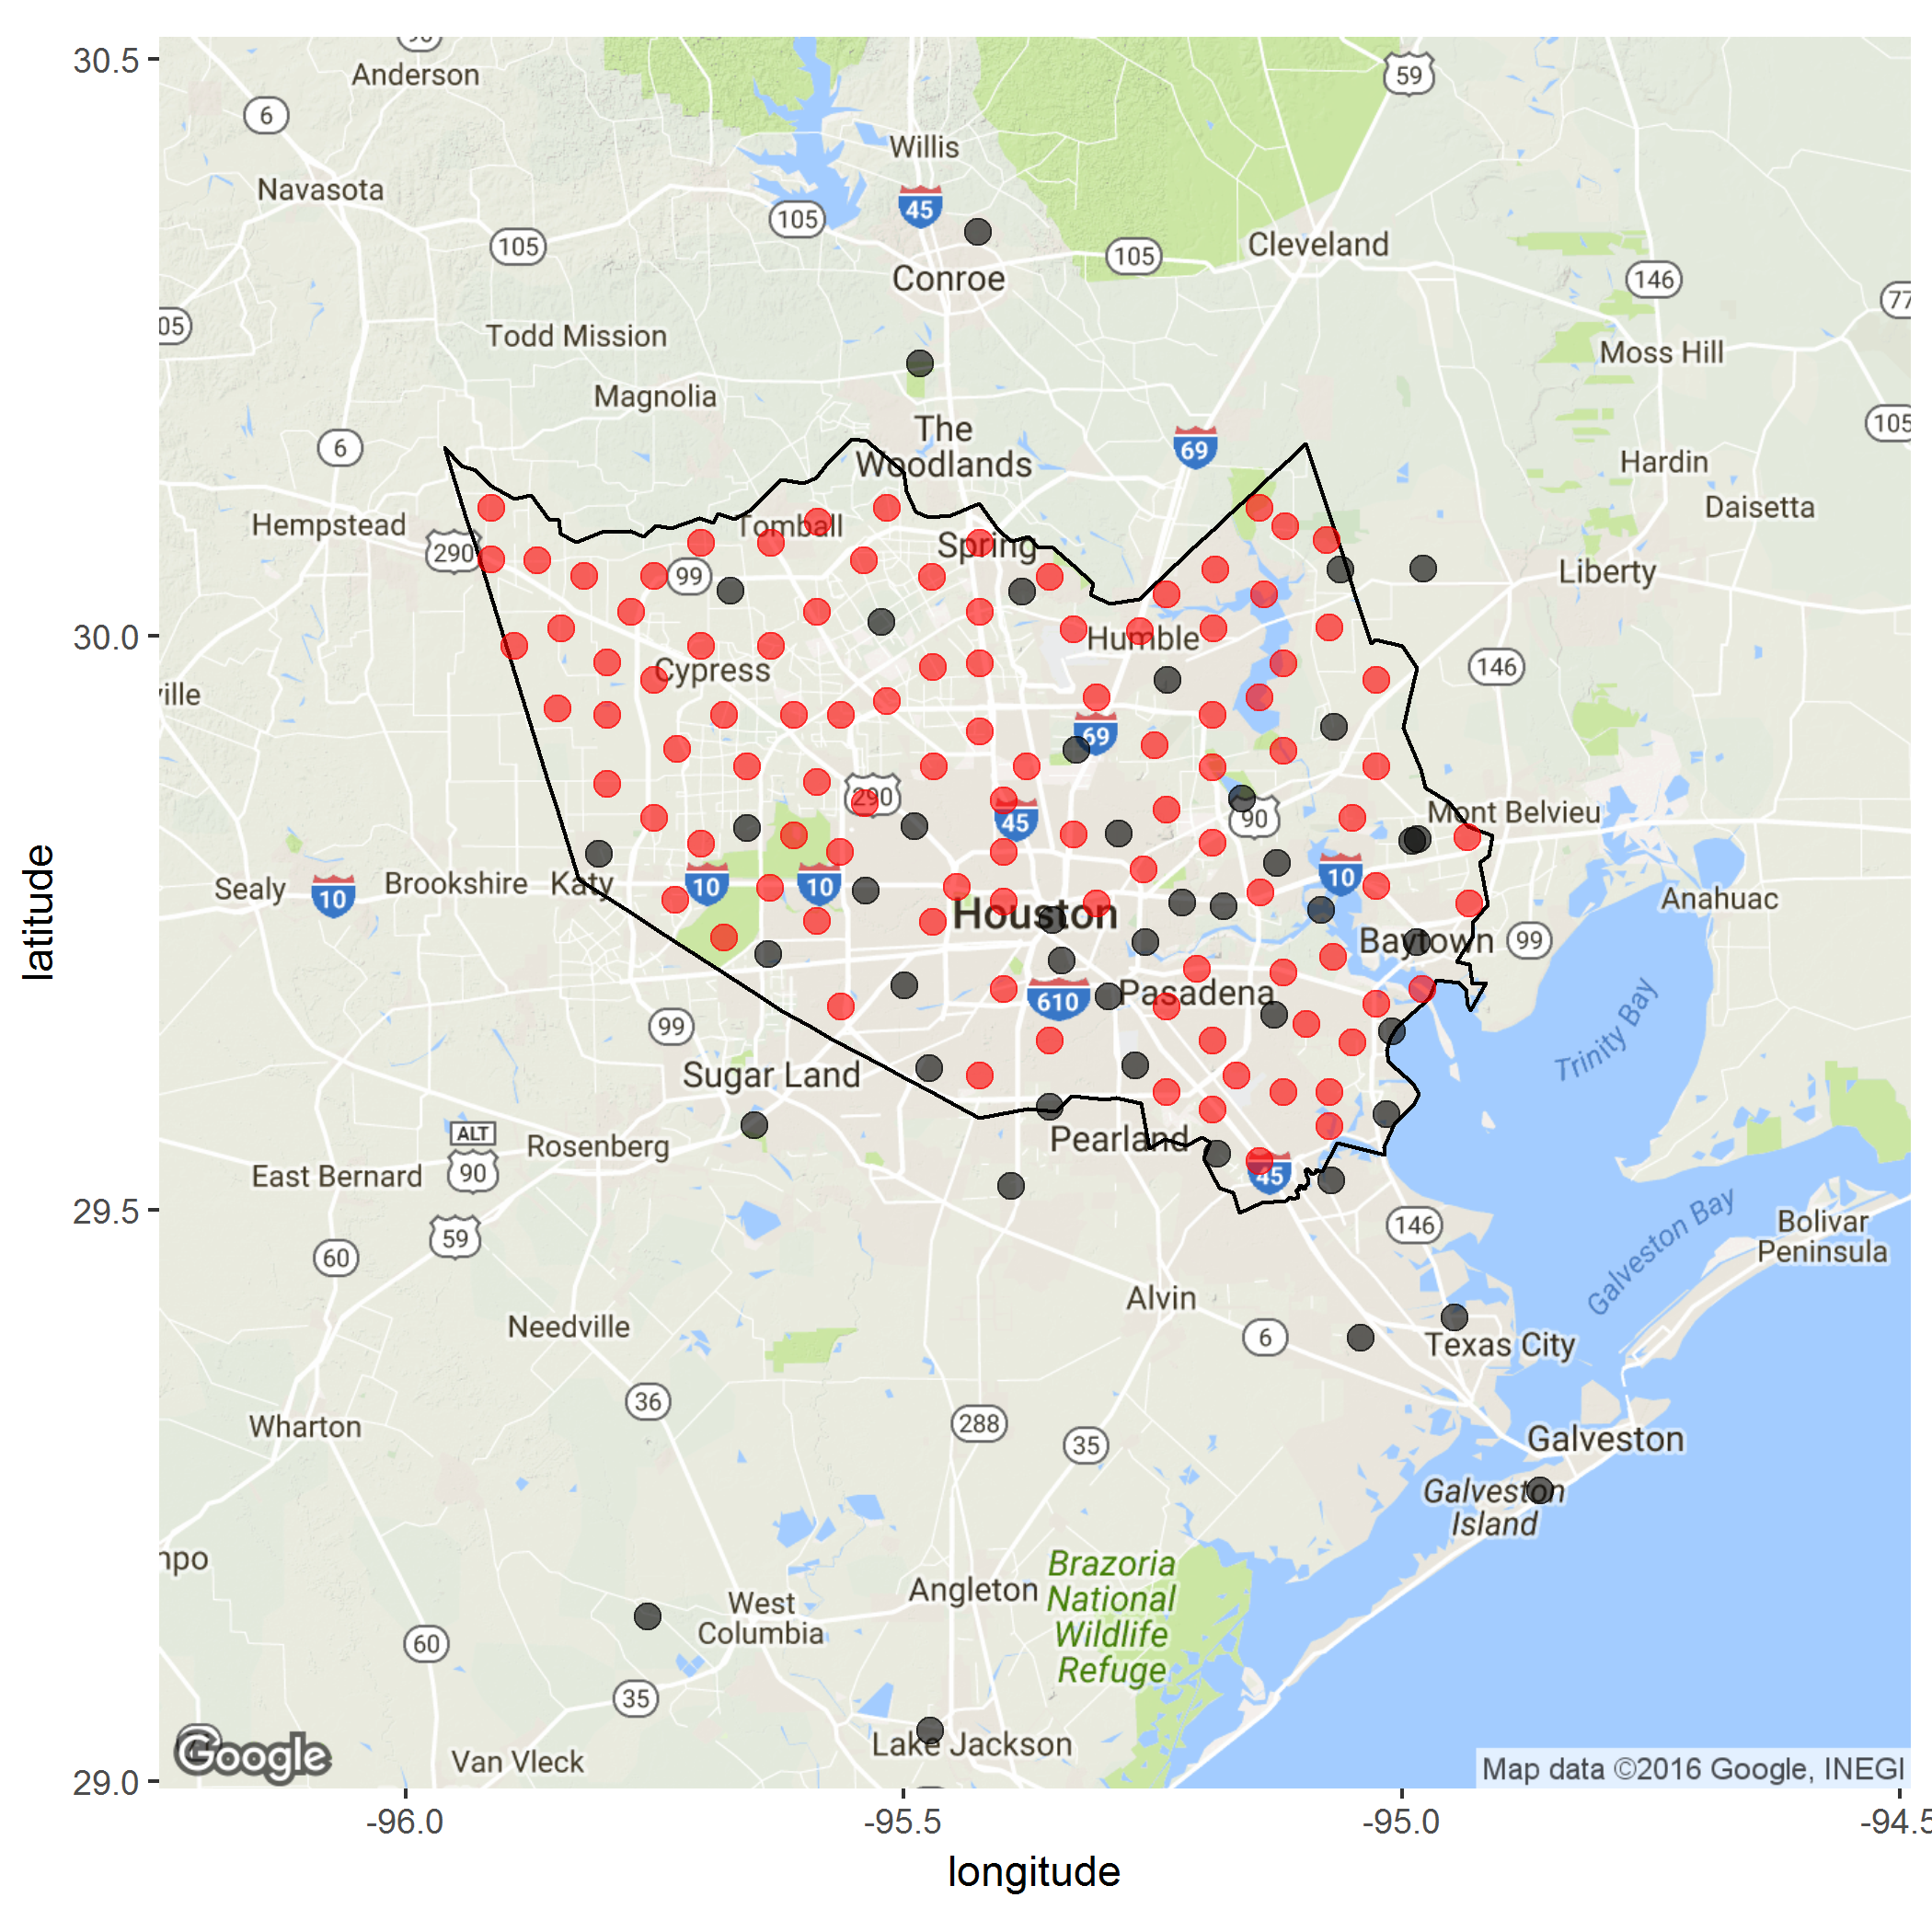
\includegraphics[scale=.35]{../code/kriging/sig2pukmean.png}
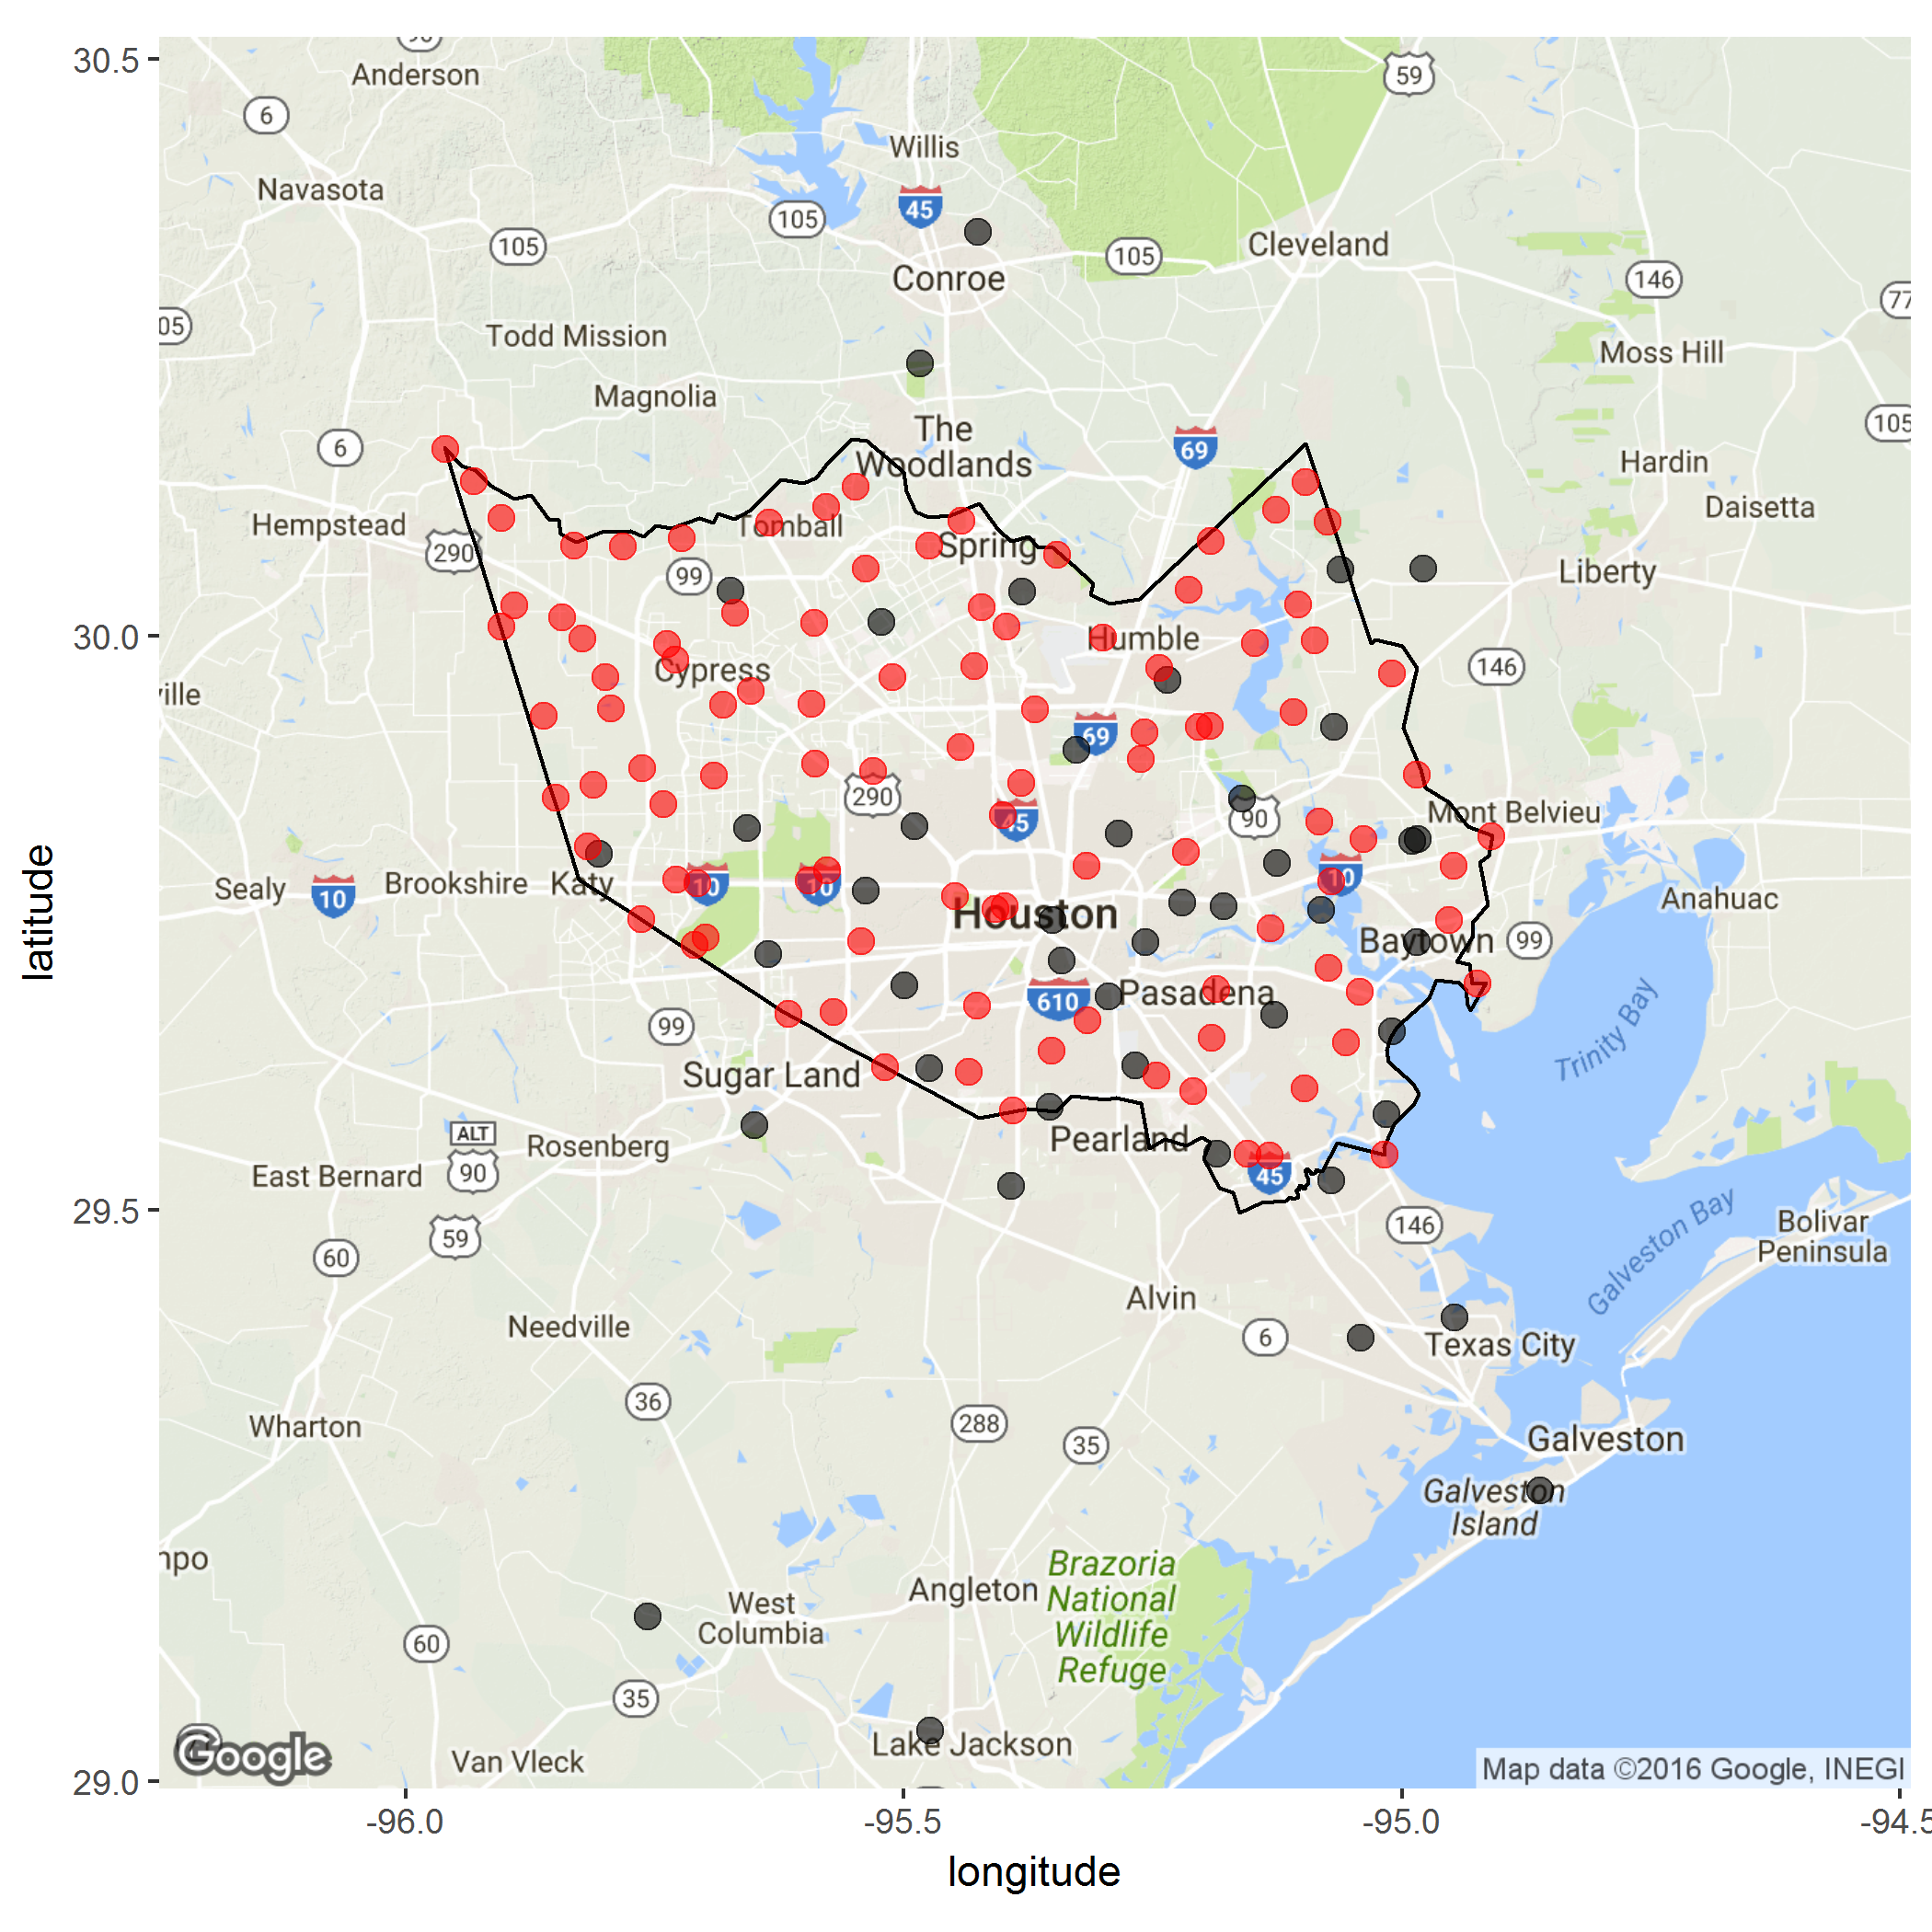
\includegraphics[scale=.35]{../code/kriging/sig2pukmax.png}
\cprotect\caption{Best designs found according to $\overline{Q}_{puk}$ (left) and $Q^*_{puk}$ (right). Original network points are grey, new points are red. Harris County is outlined in black. Map courtesy of Google Maps via \verb0ggmap0 \citep{ggmap2013}.}
\label{fig:designout}
\end{figure}

Figure \ref{fig:designout} contains the best designs found using both objective functions. When using the mean kriging variance ($\overline{Q}_{puk}$), the best design spreads nodes of the network fairly evenly throughout the spatial domain. With the maximum kriging variance ($Q^*_{puk}$), the best design is more erratic. Notably, there are many more nodes directly on or very close to the border of the spatial domain. Further, interior areas have a tendency to be more sparsely populated with nodes. This is unsurprising since $Q^*_{puk}$ is worst case kriging variance over the entire county, which incentivizes putting monitoring locations near the edges of the county for two reasons. First, a point near the center of the county is likely to have monitoring locations all around it so that it is relatively easy to predict DM8 there, while a point near an edge of the county will only have monitoring locations to one side of it. Putting more monitoring locations near the edges of the county mitigates this. Second, the farther away a point is from other monitoring locations, the more the prediction depends on the model's estimate of $\bm{\beta}$ and the less it depends on the values of nearby observations. So $Q^*_{puk}$ places a premium on a better estimate of $\bm{\beta}$, and putting more monitoring locations near the edges of the county results in smaller variances for the elements of $\widehat{\bm{\beta}}_{gls}$. 

\section{Discussion}\label{sec:discuss}
[TO BE WRITTEN]

\bibliographystyle{wb_stat}
\bibliography{../pso}
\end{document}
